\section{Результаты и обсуждение}

В рамках данной работы был разработан пайплайн, позволяющий проводить воспроизводимые эксперименты по решению проблемы фаз с помощью предложенной методологии. (\url{github.com/blackwood168/xrd_phase_ml}). В нем реализовано обучение и тестирование моделей, а также inference на реальных массивах данных и структурах кристаллических соединений. В репозитории присутствуют маленькие датасеты из сгенерированных и реальных структур малых органических молекул. Также там представлены веса обученных в работе моделей. Воспроизводимость обучения обеспечивает фиксирование начальных значений генераторов случайных состояний.

\subsubsection*{Результаты обучения}

\begin{table}[H]
\caption{Эффективность моделей до и после дообучения на синтетическом и реальном датасете}
\label{doposle}
\centering
\footnotesize
\begin{tabular}{|l|l|l|l|} 
\hline
\textbf{Model} & \textbf{Metric} & \textbf{Synth} & \textbf{CSD}  \\ 
\hline
\multirow{3}{*}{UNet} 
& Before, R & 0.477 & 0.590 \\ 
& After, R  & 0.632 & 0.393 \\ 
& $\Delta$, \%       & -32.6 & 33.4  \\
\hline
\multirow{3}{*}{FFT\_UNet}
& Before, R & 0.726 & 0.646 \\ 
& After, R  & 0.619 & \textbf{0.336} \\ 
& $\Delta$, \%       & 14.7  & 48.0  \\
\hline
\multirow{3}{*}{XRD\_Transformer}
& Before, R & 0.346 & 0.581 \\ 
& After, R  & 0.615 & 0.358 \\ 
& $\Delta$, \%       & -77.9 & 38.4  \\
\hline
\end{tabular}
\end{table}

Было проведено обучение на синтетических данных и последующее дообучение на реальных. Сравнение R-фактора для моделей до и после дообучения представлено в таблице \ref{doposle}. После дообучение на реальных данных точность предсказания моделей увеличивается минимум в 1.5 раза, однако теряют в точности на синтетических данных, кроме кастомного UNet с Фурье-преобразованием. Лучшую точность имеет модель UNet\_FFT, от которой немного отстает трансформер. В сводной таблице \ref{svod} представлены значения метрик на реальных данных финальных моделей. Таким образом, UNet\_FFT занимает меньше видеопамяти, работает быстрее и достигает лучшей метрики на тестовых реальных данных.

\begin{table}[H]
\centering
\caption{Значения метрик на тестовом реальном наборе данных моделей после дообучения}
\label{svod}
\begin{tabular}{|c|c|c|c|} 
\hline
\diagbox{\textbf{Metric}}{\textbf{Model}} & \textbf{UNet} & \textbf{FFT\_UNet} & \textbf{XRD\_Transformer}  \\ 
\hline
MSE$\cdot10^{-3}$                               & 1,39      & 1,20           & 1,31                   \\ 
\hline
R                                & 0,393         & \textbf{0,336}              & 0,358                      \\
\hline
\end{tabular}
\end{table}

\subsubsection*{Анализ моделей}

Также был проведен анализ полученных моделей. Для трансформера были построены карты внимания (рис. \ref{attention_maps}) при обработке одной из тестовых реальных структур, из которых видно, что модель в первых блоках имеет более рассеяное и равномерное внимание, что говорит о том, что сначала производится сбор общего контекста. В последующих блоках внимание становится более сфокусированным и локализованным, показывая, что модель учится выделять важные взаимосвязи. Также наблюдается способность модели связывать дальние отражения, что важно в нашей задаче. Более сильные связи наблюдается вдоль оси l; также можно заметить диагональные паттерны внимание, что соответствует систематическим погасаниям. Таким образом, можно сделать вывод, что модель научилась распрознавать кристаллографические закономерности.

\begin{figure}[H]
    \centering
    \includegraphics[width=1\textwidth]{figures/all_attention_connections.png}
    \caption{Связи внимания в блоках трансформера}
    \label{attention_maps}
\end{figure}

Также был проведен анализ первого блока моделей UNet и FFT\_UNet с помощью GradCAM (рис. \ref{gradU}, \ref{gradFFT}). По паттерну для UNet можно замтетить, что модель обращает исключительное внимание на границы дифракционной картины низкого разрешения. Смущает, что высокие значения Attribution и Overlay достигаются во всем диапазоне вне дифракционной картины на входе. Паттерн же для FFT\_UNet кажется более разумным: Attribution и Overlay распространяются на входную картину и немного за неё, что показывает, что модель ищет информацию около границы дифракционной картины. Наиболее высокие значения внимания достигаются в высокоинтенсивной зоне, дальше от неё значения монотонно спадают.

\begin{figure}[H]
    \centering
    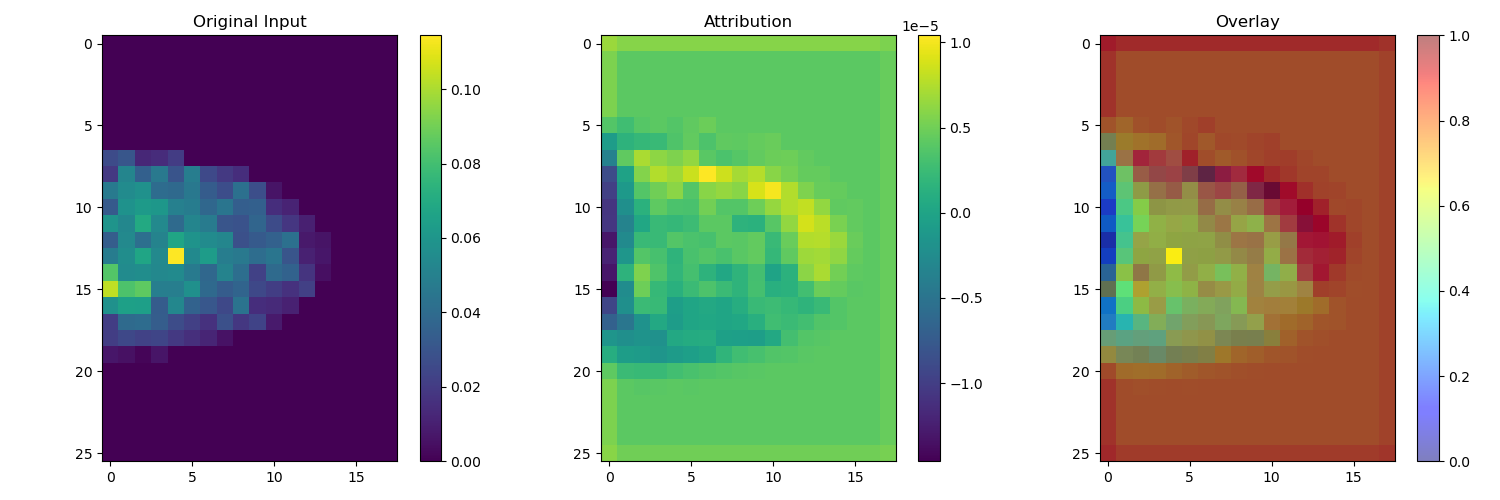
\includegraphics[width=1\textwidth]{figures/attribution_overlay.png}
    \caption{Анализ первого блока UNet с помощью GradCAM}
    \label{gradU}
\end{figure}

\begin{figure}[H]
    \centering
    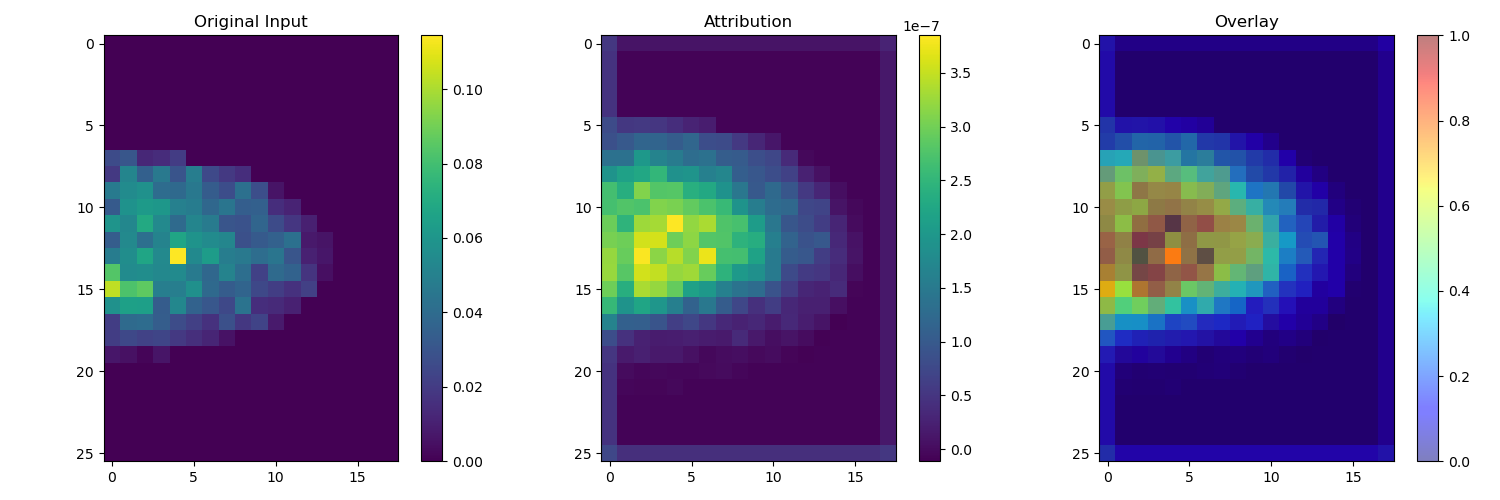
\includegraphics[width=1\textwidth]{figures/attribution_overlay_fft.png}
    \caption{Анализ первого блока FFT\_UNet с помощью GradCAM}
    \label{gradFFT}
\end{figure}

Также были получены карты чувствительности для данных моделей (рис. \ref{sens}). По ним можно сделать вывод, что модели в целом робастные и стабильно работают при добавлении шума практически во всем обратном пространстве. Однако существуют единичные воксели, которые претерпевают большие возмущения из-за шума. 


\begin{figure}[H]
    \centering
    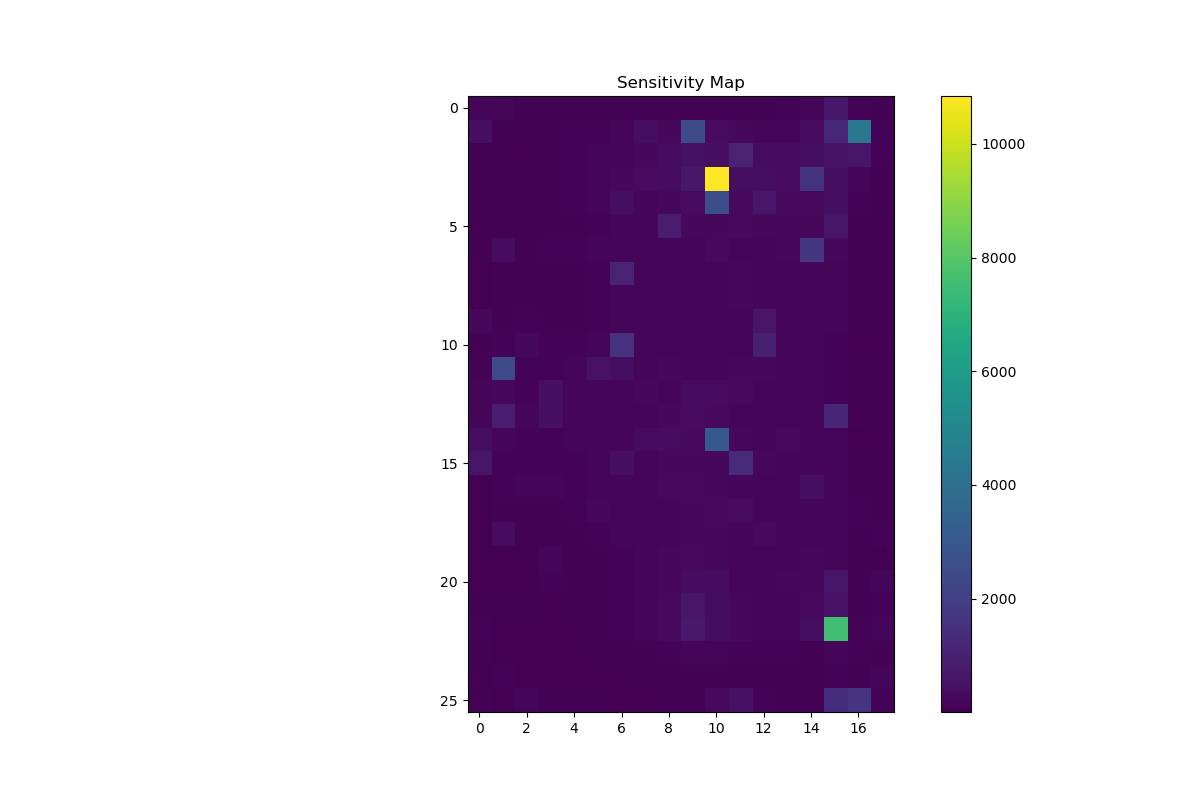
\includegraphics[width=0.5\textwidth]{figures/sensitivity_map.png}\hfill
    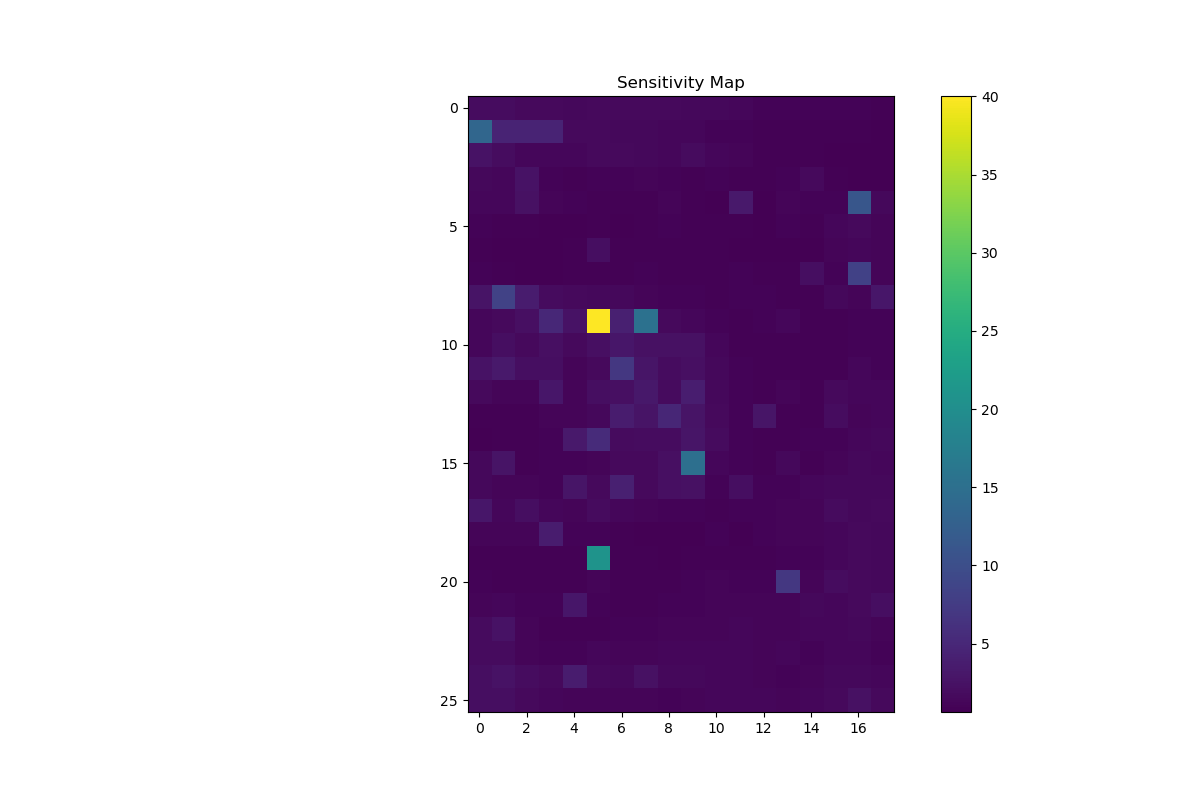
\includegraphics[width=0.5\textwidth]{figures/sensitivity_map_fft.png}
    \caption{Карты чувствительности для UNet (слева) и FFT\_UNet (справа)}
    \label{sens}
\end{figure}





\subsubsection*{Проверка на реальных данных}

Несмотря на неплохие значения метрик на реальных моноклинных структурах из Кембриджского Банка Структурных данных, качества восстановления тензора отражений недостаточно для решения структуры с помощью SHELXT. На рис. \ref{recon_ex} представлены сечения тензора отражений для реальной структуры, R-фактор восстановленного тензора с помощью FFT\_UNet равен 0.346. Нейросеть достаточно точно предсказывает границы дифракционной картины, средние значения по вокселям (если их брать по дуге) тоже достаточно близки. Но восстановленные значения в тензоре более смазанны вдоль этих дуг, картине не хватает более точного распределения амплитуд по соседним вокселям в каждой локальной области. 

\begin{figure}[H]
    \centering
    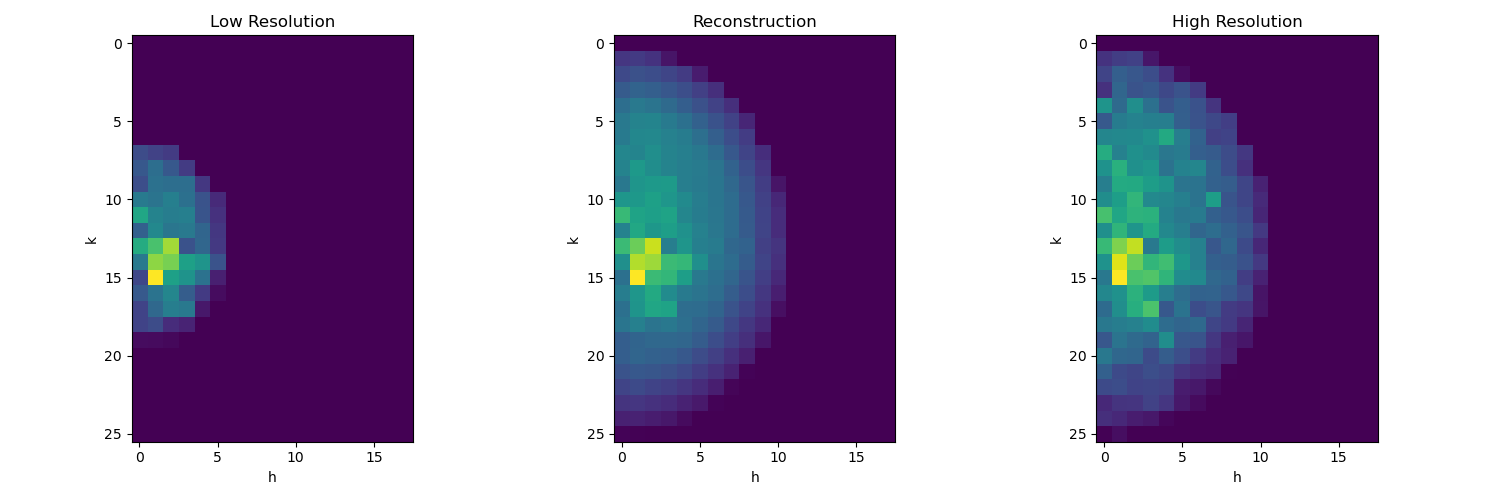
\includegraphics[width=1\textwidth]{figures/recon_example.png}
    \caption{Типичная реконструкция дифракции реальной структуры, $R = 0.346$}
    \label{recon_ex}
\end{figure}

Как уже было оговорено, дифракционные отражения не обладают локальной связанностью, и для успешного решения задачи фаз требуется очень точно определить амплитуду в каждом вокселе. Несмотря на то, что модели машинного обучения успешно схватывают кристаллографические закономерности, им не хватает более точного численного определения в каждом вокселе данных. Таким образом, методы глубокого обучения успешно определяют кристаллографические паттерны и закономерности в обратном пространстве, однако им не хватает точности для решения проблемы фаз при восстановлении численных значений амплитуд отражений.

\subsubsection*{Дальнейшие планы и предложения}

В работе было показано, что методы ИИ успешно схватывают кристаллографические закономерности, однако из-за специфики обратного пространства для решения проблемы фаз им не хватает точности. Совершив переход в локально связанное пространство, можно предположить, что нейронные сети справятся с поставленной задачей.

Для решения проблемы фаз часто используется так называемая функция Паттерсона:

\begin{center}
    $P(u, v, w) = \sum\limits_{h,k,l\in Z} |F(h,k,l)|^2e^{-2\pi i(hu+kv+lw)}$
\end{center}

Таким образом, функция Паттерсона является Фурье-преобразованием интенсивностей дифракционных максимумов, где за их фазы приняты нули. Таким образом, перейдя от тензора амплитуд/интенсивностей к трехмерной картине функции Паттерсона --- получается классическая задача Super Resolution, поскольку для дифракционной картины низкого разрешения получится Фурье-образ низкого разрешения, разрешение которого требуется повысить так, чтобы восстановленная картина соответствовала Фурье-образу дифракционной картины высокого разрешения (рис. \ref{patt}). После увеличения разрешения трехмерной картины функции Паттерсона, мы можем вернуться в обратное пространство, рассчитав интенсивности (и из них амплитуды) рентгенодифракционных отражений, и решить проблему фаз с помощью уже описанных ab initio методов.

\begin{figure}[H]
    \centering
    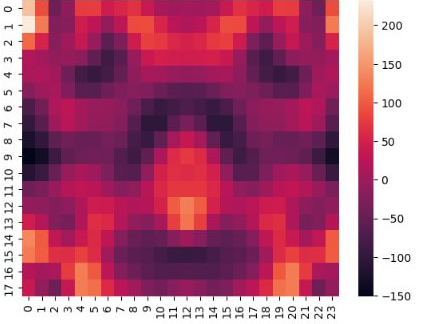
\includegraphics[width=0.5\textwidth]{figures/patt_high.png}\hfill
    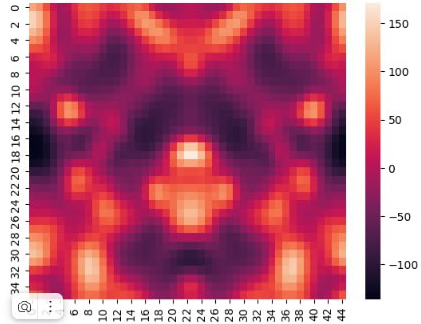
\includegraphics[width=0.5\textwidth]{figures/patt_low.png}
    \caption{Типичное сечение функции Паттерсона по данным низкого (слева) и высокого (справа) разрешения}
    \label{patt}
\end{figure}